\newlength{\plotheight}
\setlength{\plotheight}{5.8cm}

\chapter{Results and discussion}\

\section{Tabular benchmarks results}

We begin with the combined results from all tasks in Figure~\ref{ci:tabular}. It shows the average ranks of the algorithms across 15 tasks from 3 tabular benchmarks. The connecting bars signify that there is not a statistically significant difference between the algorithms within the group. From the diagram, we can observe that three distinct groups of algorithms arise. Random search ended up last in almost all tasks except for one, where it was very close, and performed statistically worse than all other algorithms. DEHB also did not perform well, as the DyHPO and the Hypertune were significantly better. The situation is not as clear on the other side of the spectrum because none of the better algorithms was consistent enough. Even DyHPO, achieving the best average rank, ended in the worst half of the algorithms on some tasks.
% TODO: Get a table with number of wins, number of 2nd places and so on.

\begin{figure}[H]
    \centering
    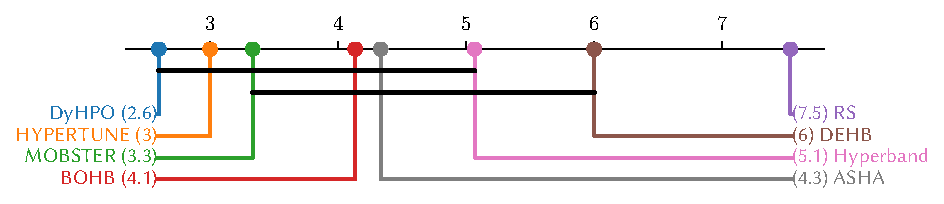
\includegraphics[scale=.75]{./img/tabular_exp/cd_diagram.pdf}
    \caption{Critical difference diagram for tabular benchmarks at the full budget. Average ranks are shown on the x-axis. Connected ranks via a bar indicate that performances are not significantly different ($p>0.05$).}
    \label{ci:tabular}
\end{figure}

For illustration purposes, we present the results of a single task in Figure~\ref{fig:parkinsons}. We provide the complete set of plots from all tasks in Appendix~\ref{ch:results_appendix}. We chose the fcnet-parkinsons task for the presentation because it allows us to show several general traits and performance of the algorithms. It is often the case in our experiments that random search is clearly behind all other algorithms, but it is catching up as the budget increases. We can also notice the fixed schedule of Hyperband. It takes Hyperband approximately 300 trials until it finally starts evaluating the first configuration fully. These delays hurt the early performance of Hyperband. In the case of FCNet with a maximal budget per configuration of 100 epochs, Hyperband should use approximately 25 full evaluations of budget per iteration. Therefore, it does not even finish the first iteration with our budget restriction. We can also notice that in the first bracket, the model-less Hyperband performs similarly to the model-based extensions. DEHB did not perform well in our experiments, it was often outperformed by model-less approaches. The performance of the most advanced methods was comparable. We cannot conclusively say that one is better than the other, as it often depends on the specific problem.

\begin{figure}
    \centering
    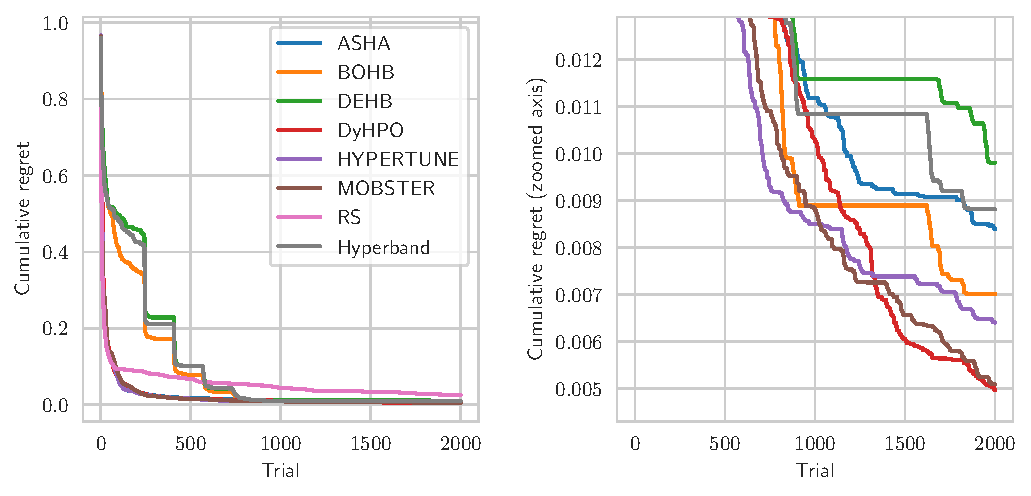
\includegraphics[scale=.75]{img/tabular_exp/fcnet-parkinsons_plot.pdf}
    \caption{The average regret over 30 runs on the fcnet-parkinsons task. On the right, we show the same results but zoomed in.}
    \label{fig:parkinsons}
\end{figure}

% Speedup factor
The key focus of this thesis is efficiency. We measure efficiency by comparing the algorithms to random search. We compute how much faster can the algorithms find a solution as good as random search has found after spending the whole budget. We call this measure the speedup factor and present the results in Table~\ref{tab:speedup}. The reported speedup factor is averaged over all benchmarks and repetitions. We assume a speedup is greater than one, which was broken for one dataset, where random search showed the best performance with a small margin. Because we do not have the data beyond the maximal budget, we have set the speedup factor to 1 in such cases. Nevertheless, the speedup factors are significant. Even the lowest reported value from any confidence interval is $3.39$ and the values of averages are around $6$ for the more advanced algorithms. The confidence intervals are overlapping for all pairs of algorithms, though.

\subfile{./tables/tab_results.tex}

% Overhead
We have seen that in terms of epochs, all advanced methods beat random search in efficiency. But that neglects the runtime, which could offset the gains. We examine the overhead in Figure~\ref{fig:overhead}. There are several things to note first. The overhead depends on the implementation. We compare all algorithms within the same framework on the same benchmark, but we have noticed there is an overhead of approximately 2 seconds when configurations change, both for a new configuration and a resumed configuration. DyHPO suffers from this kind of overhead the most because the used implementation pauses training after 2 epochs at most, even if the same configuration is immediately resumed again. That is why we see the steepest and almost linear line for DyHPO.\@ The methods based on Hyperband have the highest overhead in the beginning because they start with a bracket that tries the most configurations for the smallest budget. In the fcnet-naval example, a new configuration is sampled at each trial for the first 250 trials. From the comparison between ASHA and HyperTune, or ASHA and MOBSTER, we can see the overhead of the Bayesian surrogate model. We can notice that the slope of the overhead changes more with additional trials for the model-based algorithms than for ASHA, but the difference is not that large.
\begin{figure}
    \centering
    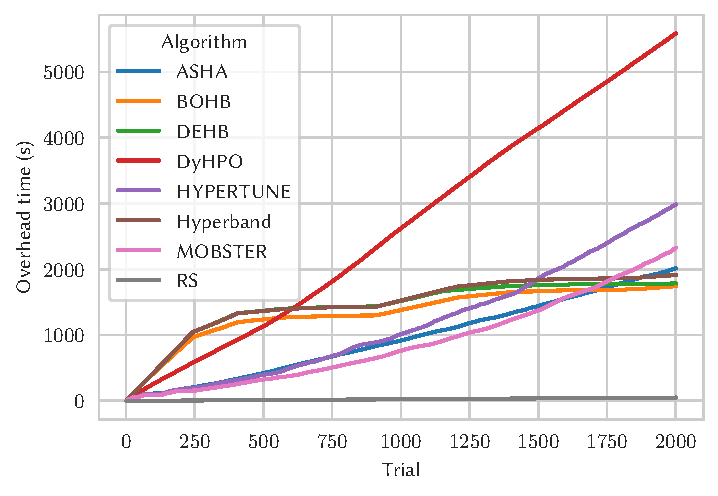
\includegraphics[scale=0.75]{./img/tabular_exp/overhead.pdf}
    \caption{Overhead on FCNet Naval benchmark.}
    \label{fig:overhead}
\end{figure}

% Heatmap
In order to estimate the reliability and consistency of the methods, we provide the heatmap of sample standard deviations (SD) in Figure~\ref{fig:heatmap}. The SDs are normalized across tasks because we are interested in a relative comparison between the algorithms, not in the actual magnitudes. We can see that random search has the largest SD in almost all tasks. Interestingly, it has the smallest SD in the lcbench-covertype tasks. After closer inspection of the results, one possible explanation might be that all algorithms struggle to consistently find a good solution. Although random search achieved the best SD, its results on that task were the worst by a large margin. In other words, its SD is probably low because it fails to find a good solution most of the time, unlike the other algorithms that are more successful. DyHPO even has the second-best SD on lcbench-covertype, and achieved the best results by a large margin.

The most pronounced differences between the worst and the best algorithms can be noticed in the FCNet tasks. Nevertheless, there are not many other obvious patterns in the data. HyperTune and MOBSTER seem to be the most consistent in FCNet tasks overall, and they also do well in NAS-Bench tasks, even if we consider the results. In LCBench tasks, DyHPO seems to be one of the most consistent algorithms on average, but its SD is high on the \textit{albert} and the \textit{christine} datasets. It might be the most useful to compare the average standard deviation across all tasks. DyHPO has the lowest mean SD, followed closely by ASHA, with HyperTune in third place. The other algorithms are also not far behind. DEHB is second to last, and random search is last.

\begin{figure}[H]
    \centering
    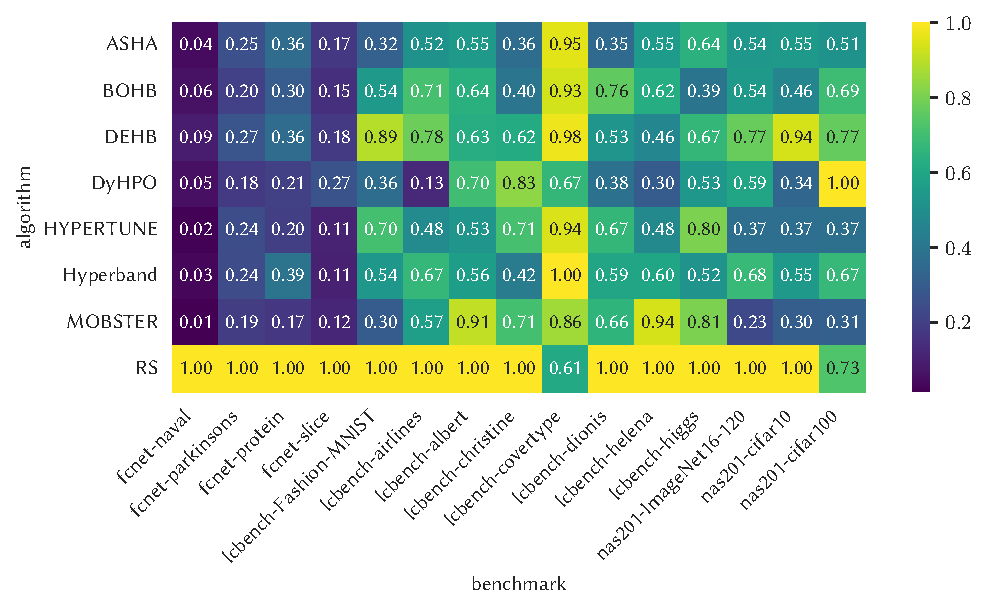
\includegraphics[scale=0.75]{img/tabular_exp/stds_heatmap.pdf}
    \caption{The heatmap of sample standard deviations of the best results found, averaged over 30 repetitions. The standard deviations are normalized for each task.}
    \label{fig:heatmap}
\end{figure}


\section{Real-world experiments results}

First, we present the combined results from all real-world experiments (Figure~\ref{fig:real_combined}). As anticipated, seven experiments are not enough for a~reliable statistical analysis. Nevertheless, the average ranks are still worth examining. The order of algorithms is very similar to the results from tabular benchmarks. The only difference at a \SI{100}{\percent} budget is that ASHA overtook BOHB on real-world tasks. Another thing to notice is that HyperTune performed better than DyHPO at a \SI{50}{\percent} budget, even though this difference is minor. Next, we will review the results for each experiment individually.


\begin{figure}[H]
    \begin{subfigure}{.5\textwidth}
        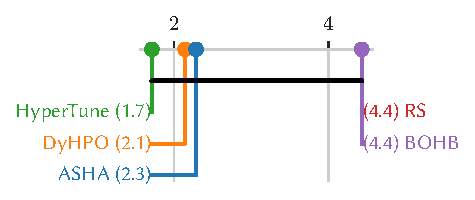
\includegraphics[width=.92\textwidth]{img/real_exp/cd_diagram_real_half.pdf}%
        \caption{At \SI{50}{\percent} budget.}%
        %\label{fig:second}
    \end{subfigure}%
    \begin{subfigure}{.5\textwidth}
        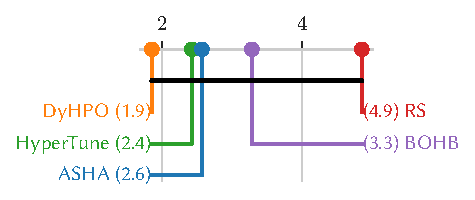
\includegraphics[width=.92\textwidth]{img/real_exp/cd_diagram_real.pdf}%
        \caption{At \SI{100}{\percent} budget.}%
        %\label{fig:first}
    \end{subfigure}%
\caption{Critical difference diagrams for real-world experiments at two budget levels. Average ranks are shown on the x-axis. All algorithms are connected via a bar, which indicates that performances are not significantly different ($p>0.05$).}
\label{fig:real_combined}
\end{figure}

%\subsection{Evaluation}
%\subsection{Experimental Setup}


%\begin{figure}[H]
%    \centering
%    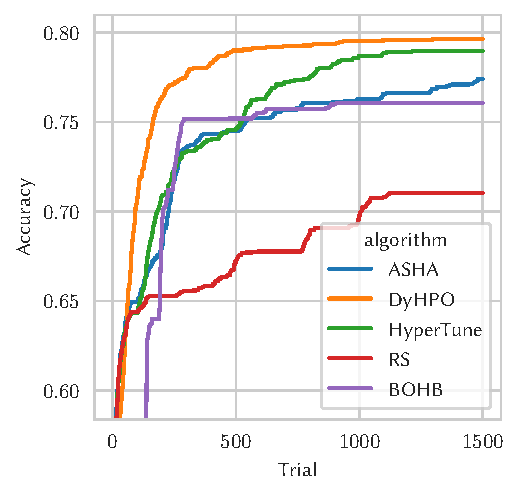
\includegraphics[scale=0.58]{img/real_exp/cifar10_simple_plot.pdf}
%    \caption{CNN network trained on CIFAR10 dataset for 20 full evaluations.}
%    \label{fig:cifar10}
%\end{figure}

%\subfile{./tables/cifar10_simple_results.tex}

%\subfile{./tables/cifar10_simple_results_short.tex}

%
%\begin{figure}[H]
%    \centering
%    \begin{minipage}[b]{2.5in}
%        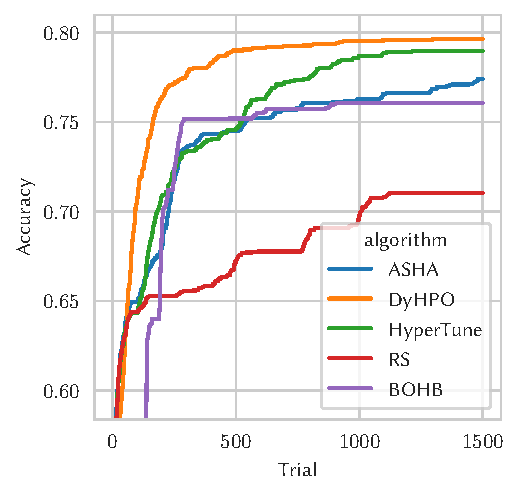
\includegraphics[width=\linewidth]{img/real_exp/cifar10_simple_plot.pdf}
%        \caption{Your Plot Caption}
%    \end{minipage}
%    \hfill
%    \begin{minipage}[b]{2.5in}
%        \input{./tables/cifar10_simple_results_short.tex}
%        \caption{Your Table Caption}
%    \end{minipage}
%\end{figure}
%

\subsubsection{1.\ cifar10-cnn}
In the first experiment, the differences between the algorithms are the most pronounced (see Figure~\ref{fig:simple_cifar}). Indeed, using the Kruskal-Wallis test we can reject the null hypothesis and conclude that there is a statistically significant difference in the medians of the groups at both budgets. Random search is far behind the other algorithms, especially early in the search. At full budget, some solutions found by random search get close to the better-performing algorithms, but not reliably. We use Dunn's test to reject the null hypothesis for random search and DyHPO, and random search and HyperTune at both budgets, concluding there is a statistically significant difference between the algorithms. DyHPO dominates the early stage of the search, especially when compared to ASHA and BOHB, which do not achieve at \SI{100}{\percent} of the budget results that DyHPO achieves at \SI{50}{\percent} of the budget. The differences between DyHPO and ASHA with BOHB are also statistically significant for both budgets. Finally, HyperTune is significantly better than BOHB at full budget.

\begin{figure}[H]
    \begin{subfigure}{.47\textwidth}
        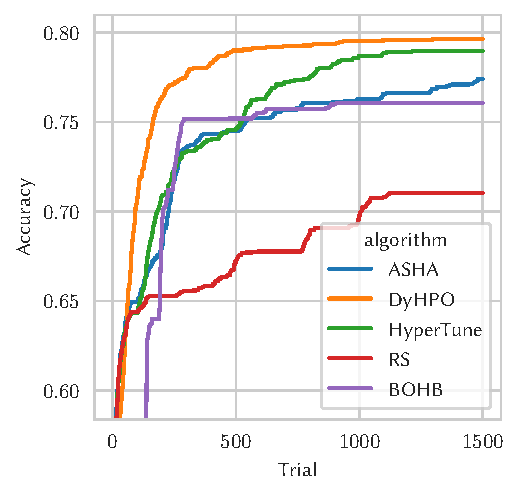
\includegraphics[height=\plotheight]{img/real_exp/cifar10_simple_plot.pdf}%
        \caption{Cumulative accuracy.}%
        %\label{fig:first}
    \end{subfigure}%
    \begin{subfigure}{.26\textwidth}
        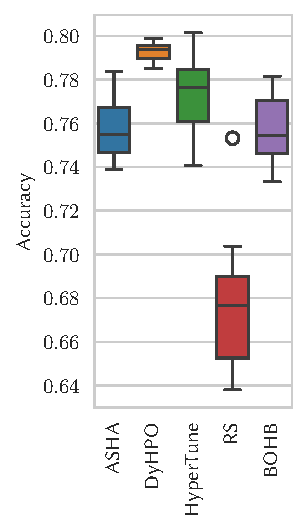
\includegraphics[height=\plotheight]{img/real_exp/cifar10_simple_boxplot_half.pdf}%
        \caption{At \SI{50}{\percent} budget.}%
        %\label{fig:second}
    \end{subfigure}%
    \begin{subfigure}{.26\textwidth}
        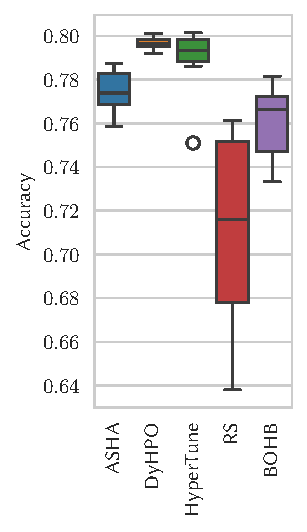
\includegraphics[height=\plotheight]{img/real_exp/cifar10_simple_boxplot_full.pdf}%
        \caption{At \SI{100}{\percent} budget.}%
        %\label{fig:second}
    \end{subfigure}%
\caption{Results of the cifar10-cnn experiment.}
\label{fig:simple_cifar}
\end{figure}

\subsubsection{2.\ cifar10-residual}
We can notice that residual CNN architecture performs much better than the simpler CNN architecture from the previous experiment, even very early in the search (see Figure~\ref{fig:resnet_cifar10}). On the other hand, the differences between hyperparameter optimization algorithms are small. A Kruskal-Wallis test resulted in a p-value of $0.51$ at a \SI{100}{\percent} budget and $0.20$ at a \SI{50}{\percent} budget, both of which are greater than the significance level of $0.05$. Therefore, we fail to reject the null hypothesis and conclude that there is no statistically significant difference in the medians of the groups at both budgets. With that said, BOHB achieved the best median and mean result on a full budget, even though not significantly better. Also, ASHA found a solution with over \SI{90}{\percent} accuracy in each run, which cannot be said for the other algorithms.

\begin{figure}[H]
    \begin{subfigure}{.47\textwidth}
        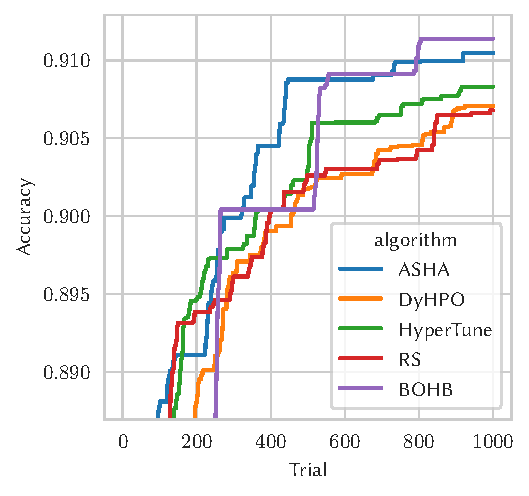
\includegraphics[height=\plotheight]{img/real_exp/cifar10_residual_plot.pdf}%
        \caption{Cumulative accuracy.}%
        %\label{fig:first}
    \end{subfigure}%
    \begin{subfigure}{.26\textwidth}
        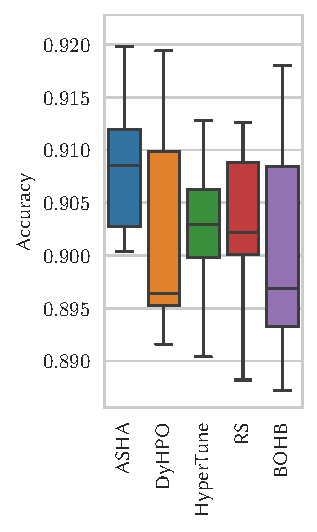
\includegraphics[height=\plotheight]{img/real_exp/cifar10_residual_boxplot_half.pdf}%
        \caption{At \SI{50}{\percent} budget.}%
        %\label{fig:second}
    \end{subfigure}%
    \begin{subfigure}{.26\textwidth}
        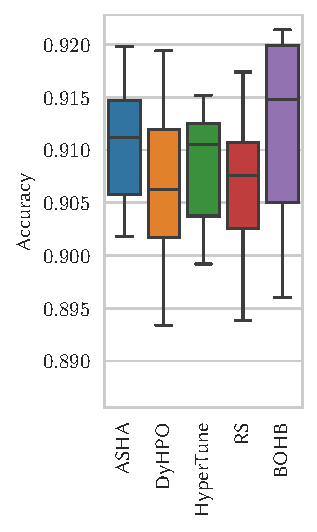
\includegraphics[height=\plotheight]{img/real_exp/cifar10_residual_boxplot_full.pdf}%
        \caption{At \SI{100}{\percent} budget.}%
        %\label{fig:second}
    \end{subfigure}%
\caption{Results of the cifar10-residual experiment.}
\label{fig:resnet_cifar10}
\end{figure}

\subsubsection{3.\ svhn-cnn}
Except for the dataset, this experiment is identical to the first experiment. The results of this experiment also resemble the results of the first experiment (see Figure~\ref{fig:simple_svhn}), but there are some differences. Most notably, DyHPO seemed to do better in the first experiment, and it is more in line with the other algorithms here. Kruskal-Wallis test rejects the null hypothesis for both budgets. Therefore, we follow up with Dunn's test. At \SI{50}{\percent} of the budget, all algorithms significantly outperform random search. By~contrast, the performance of other algorithms seems to be almost identical at a \SI{50}{\percent} budget. At full budget, the null hypothesis cannot be rejected for random search with ASHA, and random search with BOHB.\@ On the other hand, HyperTune and DyHPO did perform significantly better than random search. There is a statistically significant difference between DyHPO and BOHB, too.\@ We can also notice that DyHPO and HyperTune were both more consistent in finding a good solution than other algorithms.

\begin{figure}[H]
    \begin{subfigure}{.47\textwidth}
        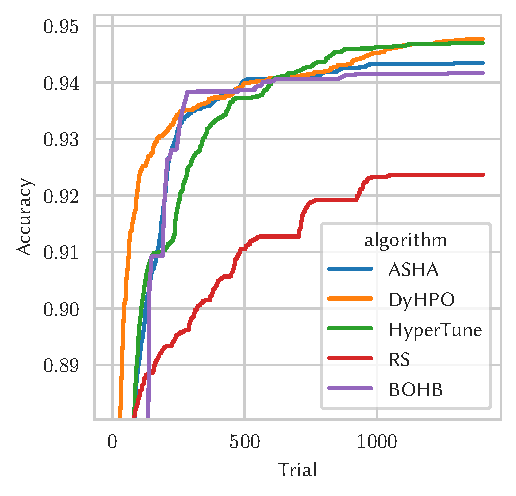
\includegraphics[height=\plotheight]{img/real_exp/svhn_simple_plot.pdf}%
        \caption{Cumulative accuracy.}%
        %\label{fig:first}
    \end{subfigure}%
    \begin{subfigure}{.26\textwidth}
        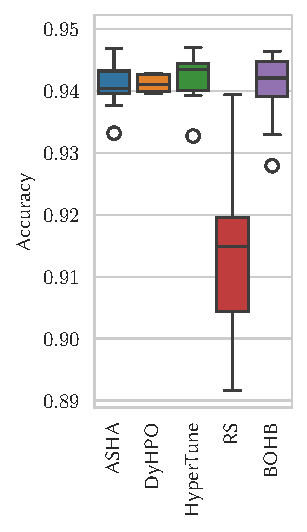
\includegraphics[height=\plotheight]{img/real_exp/svhn_simple_boxplot_half.pdf}%
        \caption{At \SI{50}{\percent} budget.}%
        %\label{fig:second}
    \end{subfigure}%
    \begin{subfigure}{.26\textwidth}
        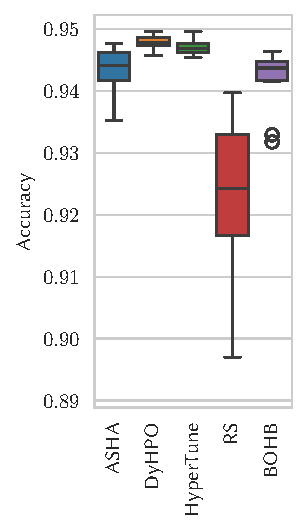
\includegraphics[height=\plotheight]{img/real_exp/svhn_simple_boxplot_full.pdf}%
        \caption{At \SI{100}{\percent} budget.}%
        %\label{fig:second}
    \end{subfigure}%
\caption{Results of the svhn-cnn experiment.}
\label{fig:simple_svhn}
\end{figure}


\subsubsection{4.\ svhn-residual}
Again, we see the importance of choosing the right architecture if we compare the results between this and the previous experiment. The results of a random search in this experiment (see Figure~\ref{fig:resnet_svhn}) start where the best networks from the previous experiment end. Kruskal-Wallis test results in p-values far below the significance level for both budgets, so we reject both null hypotheses. Dunn's pairwise comparison test points out significant differences between random search and all other algorithms on both budgets, except for ASHA at a \SI{50}{\percent} budget and BOHB at a \SI{100}{\percent} budget. The null hypothesis cannot be rejected for the other pairwise comparisons, though. DyHPO seems to offer the best anytime performance, as well as the full-budget performance, albeit with a small margin. Other algorithms are very close behind DyHPO.\@ Again, random search has the largest variance, especially on half of the budget.

\begin{figure}[H]
    \begin{subfigure}{.47\textwidth}
        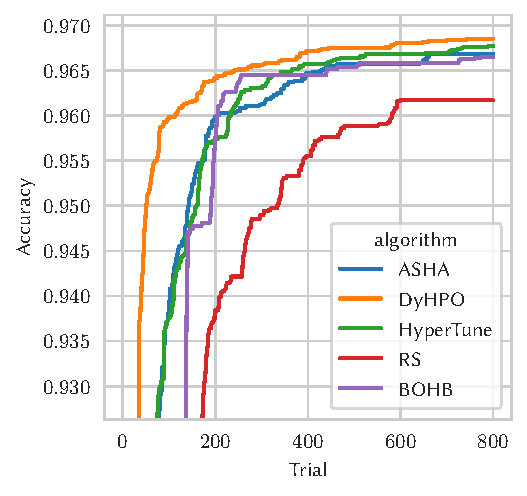
\includegraphics[height=\plotheight]{img/real_exp/svhn_residual_plot.pdf}%
        \caption{Cumulative accuracy.}%
        %\label{fig:first}
    \end{subfigure}%
    \begin{subfigure}{.26\textwidth}
        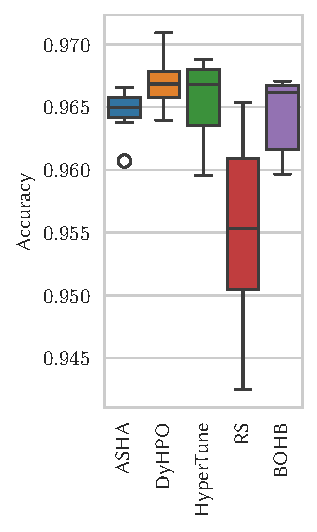
\includegraphics[height=\plotheight]{img/real_exp/svhn_residual_boxplot_half.pdf}%
        \caption{At \SI{50}{\percent} budget.}%
        %\label{fig:second}
    \end{subfigure}%
    \begin{subfigure}{.26\textwidth}
        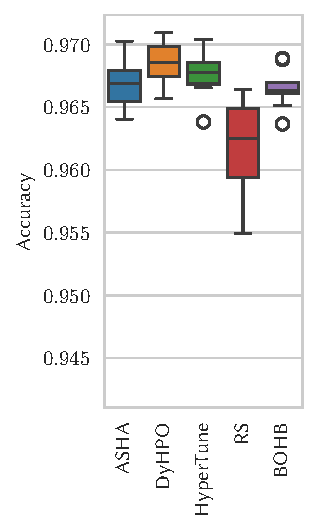
\includegraphics[height=\plotheight]{img/real_exp/svhn_residual_boxplot_full.pdf}%
        \caption{At \SI{100}{\percent} budget.}%
        %\label{fig:second}
    \end{subfigure}%
\caption{Results of the svhn-residual experiment.}
\label{fig:resnet_svhn}
\end{figure}


\subsubsection{5.\ ptbxl-rnn}
% NO significant differences at both budgets
We conducted a Kruskal-Wallis test, which resulted in p-values $0.13$ and $0.36$ at a full budget, and a half budget respectively. Therefore, we cannot reject the null hypothesis for both budgets. All methods achieved very similar results (see Figure~\ref{fig:rnn_ptbxl}); and it is not possible to tell if any method is better than the other. We can notice that the solutions found on half of the budget are only marginally worse than solutions found on the full budget. Also, the variance of the results is similar for all algorithms including random search. If any differences can be found, DyHPO has a slightly larger variance than other algorithms on both budgets.

\begin{figure}[H]
    \begin{subfigure}{.47\textwidth}
        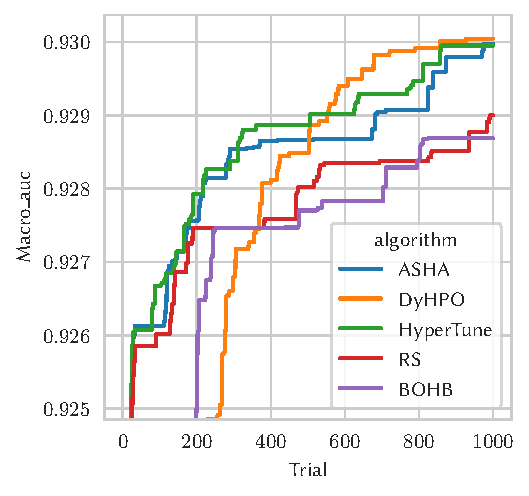
\includegraphics[height=\plotheight]{img/real_exp/ptbxl_rnn_plot.pdf}%
        \caption{Cumulative averaged ROC AUC score.}%
        %\label{fig:first}
    \end{subfigure}%
    \begin{subfigure}{.26\textwidth}
        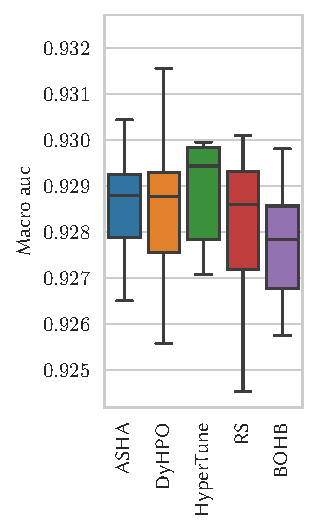
\includegraphics[height=\plotheight]{img/real_exp/ptbxl_rnn_boxplot_half.pdf}%
        \caption{At \SI{50}{\percent} budget.}%
        %\label{fig:second}
    \end{subfigure}%
    \begin{subfigure}{.26\textwidth}
        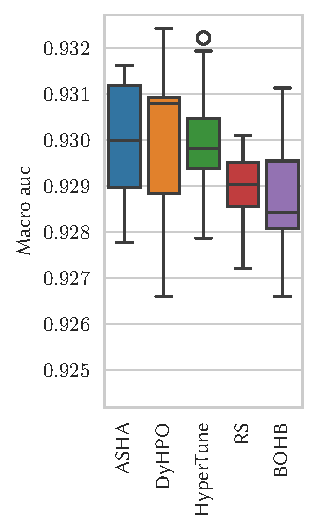
\includegraphics[height=\plotheight]{img/real_exp/ptbxl_rnn_boxplot_full.pdf}%
        \caption{At \SI{100}{\percent} budget.}%
        %\label{fig:second}
    \end{subfigure}%
\caption{Results of the ptbxl-rnn experiment.}
\label{fig:rnn_ptbxl}
\end{figure}


\subsubsection{6.\ ptbxl-xResnet1d}
% NO differences at 100, some differences at 50
In spite of the fact that xResnet1d was the best-performing architecture on the PTB-XL dataset according to the literature~\cite{strodthoff2020deep}, it seems to perform a little worse than RNN in our experiments (see Figure~\ref{fig:xresnet_ptbxl}). There is a small overlap between the results of the two architectures, though. Kruskal-Wallis test rejected the null hypothesis on both budgets. However, the follow-up Dunn's test did not find any significant differences at the full budget. At a \SI{50}{\percent} of the budget, the null hypothesis can be rejected for many pairs. Random search performed significantly worse than HyperTune and ASHA.\@ HyperTune and ASHA are indistinguishable statistically, but both performed better than all other algorithms at a \SI{50}{\percent} budget. One more thing to note is that random search has a much larger variance than other methods on half of the budget.

\begin{figure}[H]
    \begin{subfigure}{.47\textwidth}
        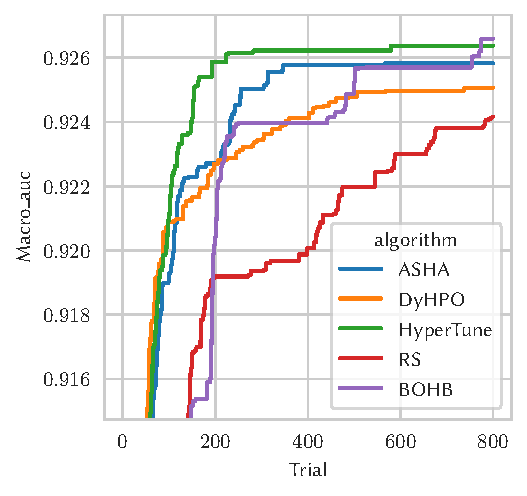
\includegraphics[height=\plotheight]{img/real_exp/ptbxl_xResNet1d_plot.pdf}%
        \caption{Cumulative averaged ROC AUC score.}%
        %\label{fig:first}
    \end{subfigure}%
    \begin{subfigure}{.26\textwidth}
        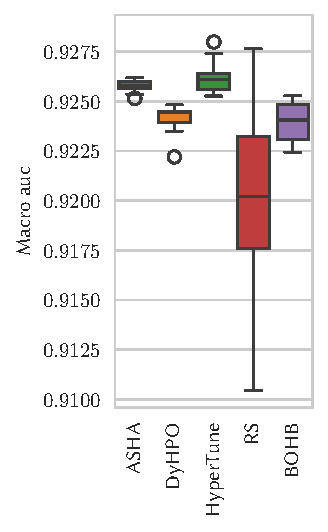
\includegraphics[height=\plotheight]{img/real_exp/ptbxl_xResNet1d_boxplot_half.pdf}%
        \caption{At \SI{50}{\percent} budget.}%
        %\label{fig:second}
    \end{subfigure}%
    \begin{subfigure}{.26\textwidth}
        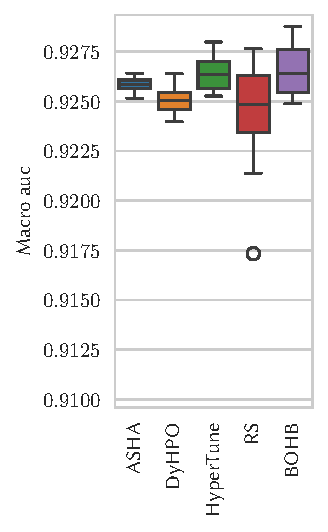
\includegraphics[height=\plotheight]{img/real_exp/ptbxl_xResNet1d_boxplot_full.pdf}%
        \caption{At \SI{100}{\percent} budget.}%
        %\label{fig:second}
    \end{subfigure}%
\caption{Results of the ptbxl-xResnet1d experiment.}
\label{fig:xresnet_ptbxl}
\end{figure}


\subsubsection{7.\ xray-densenet}
% RS DyHpo different at full budget, NO differences at 50%
The last experiment was performed on the ChestX-ray14 dataset. The p-values of Kruskal-Wallis tests are $0.02$ at a \SI{100}{\percent} budget, and $0.09$ at a \SI{100}{\percent} budget. Therefore, we can reject the null hypothesis at the full budget only. Dunn's test found a significant difference only for the DyHPO and random search pair, where DyHPO performed significantly better than random search. The other results are very close (see Figure~\ref{fig:densenet_chestx}). ASHA seems to be slightly better at half of the budget than the other algorithms except for DyHPO, but then it barely improves until the end. The random search did well in this experiment, too, considering that it is comparable to the other algorithms.

\begin{figure}[H]
    \begin{subfigure}{.47\textwidth}
        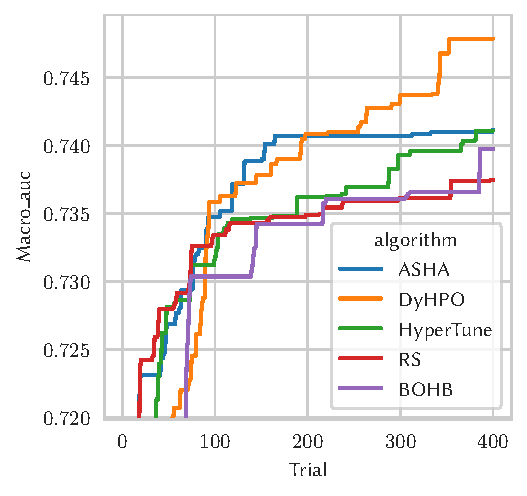
\includegraphics[height=\plotheight]{img/real_exp/xray_densenet_plot.pdf}%
        \caption{Cumulative averaged ROC AUC score.}%
        %\label{fig:first}
    \end{subfigure}%
    \begin{subfigure}{.26\textwidth}
        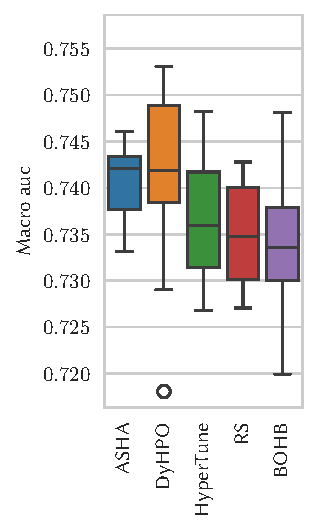
\includegraphics[height=\plotheight]{img/real_exp/xray_densenet_boxplot_half.pdf}%
        \caption{At \SI{50}{\percent} budget.}%
        %\label{fig:second}
    \end{subfigure}%
    \begin{subfigure}{.26\textwidth}
        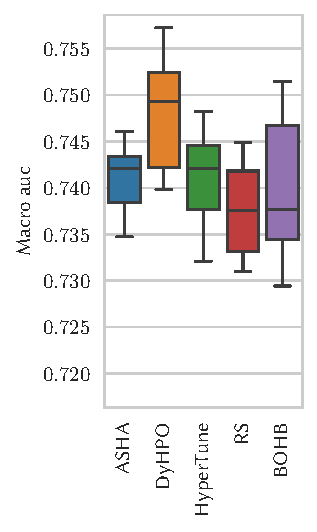
\includegraphics[height=\plotheight]{img/real_exp/xray_densenet_boxplot_full.pdf}%
        \caption{At \SI{100}{\percent} budget.}%
        %\label{fig:second}
    \end{subfigure}%
\caption{Results of the xray-densenet experiment.}
\label{fig:densenet_chestx}
\end{figure}


% \clearpage
\section{Discussion} % Interpret and explain my results

% Restate your research problem and research questions

% Summary of key findings

    % the data suggest that..
    % the data support/oppose the theory that..
    % the analysis identifies..

% Interpretation of results
% More detailed findigs

% Speedup factor and inconsistency
The data suggest advanced algorithms can find a good solution much faster than random search. In tabular experiments, the average speedup factor of algorithms over random search was approximately in the range of $4.5$ for DEHB and Hyperband, to $7$ for DyHPO.\@ Meaning that DyHPO found a solution as good as the random search, but only using a $1/7$th of the budget on average. There was just a single task out of the fifteen, where random search was comparable to the other algorithms. Another important thing to consider is that random search is less consistent. We have observed that the spread of the results can be many times larger for random search, in addition to usually being worse on average. The data suggest that if there is just one opportunity to optimize the hyperparameters or the budget is very limited, a random search will not find a good solution reliably.
% Did we?

% Real-world architectures - large differences on CNN
The results from real-world experiments were more diverse. We have seen the largest differences between algorithms on the simplest architecture. We think that the hyperparameters probably had a larger effect on the small CNN network than on the large and complex networks, because the large networks have a large capacity overhead and also use techniques like residual connections to make learning easier. Take the xResnet1d as an example. From the individual runs we have found that all three network sizes were able to achieve over $0.925$ ROC AUC score, which is very close to the best achieved result, suggesting that the size of the network alone did not have much influence over the performance.

We have found no statistically significant differences between algorithms in cifar10-residual and ptbxl-rnn experiments, which illustrates that some tasks might not even benefit from an advanced hyperparameter tuning algorithm. Nevertheless, there were significant differences in all the other experiments. Most often, random search performed significantly worse than DyHPO and HyperTune. Since the ranking of the algorithms is mostly consistent with ranking in tabular experiments, we think that more differences could be found; we just do not have enough data to support it.

% Mention healthcare datasets


% Comparison with previous work

% Maybe todo? Practical implications


% Recommendations
From the research, we have several recommendations. We recommend using random search in the exploratory phase when the goal is to gain as much insight into the problem as possible. If the goal is to optimize hyperparameters efficiently, we think it is better to avoid random search. Especially ASHA sped up the search almost as much as the best algorithms without any of the downsides. It is easy to implement, parallelization is simple, and it does not even require checkpointing in the stopping variant. Moreover, the lack of a model makes it robust, as the new suggestions are always going to be randomly sampled. If the extra efficiency is needed, we recommend either DyHPO or HyperTune. DyHPO seemed to perform a little better overall, but it pauses and resumes trials much more often. Therefore, if resuming trials is expensive, we would recommend HyperTune over DyHPO.\@

We also want to point out that while the original goal was to implement a new method based on the findings of our experiments, in the end, we decided to focus exclusively on the experimental comparison, as we found out that there are no independent comparisons in the literature that we are aware of. Such comparisons are needed to uncover the strengths and weaknesses of the existing methods before new methods can be designed. Moreover, this kind of research helps practitioners pick the right algorithm, as it provides new data and eliminates the need to go through multiple articles to understand different methods and their performance.


% One of the barriers to the widespread adoption of hyperparameter optimization algorithms is the lack of empirical evidence to decide which algorithm to choose. We performed a set of experiments, both on tabular benchmarks and on real-world problems, in order to provide more data and to help practitioners with the decision of choosing a suitable hyperparameter optimization algorithm for the task at hand.
